\documentclass[a4paper,12pt]{report}
\usepackage[T2A]{fontenc}
\usepackage[utf8]{inputenc}
\usepackage[english,russian]{babel}
\usepackage{graphicx}
\usepackage{wrapfig}
\usepackage{mathtext} 				% русские буквы в фомулах
\usepackage{amsmath,amsfonts,amssymb,amsthm,mathtools} % AMS
\usepackage{icomma} % "Умная" запятая: $0,2$ --- число, $0, 2$ --- перечисление
\usepackage{capt-of}
\usepackage{appendix}
\usepackage{multirow}
\usepackage{hyperref}
\usepackage{floatrow}
\usepackage[left=2cm,right=2cm,
    top=2cm,bottom=2cm,bindingoffset=0cm]{geometry}
\usepackage{multicol} % Несколько колонок
\usepackage{gensymb}
\title{Отчёт по лабораторной работе №6.11.1

Определение ширины запрещенной зоны полупроводника}
\author{Плюскова Н.А. Б04-004 }
\date{\today}

\begin{document}

\maketitle

\section*{1. Аннотация}

В работе исследуется температурная зависимость проводимости типичного полупроводника - германия или кремния. Исследуется зависимость $\sigma(T)$ с помощью универсального цифрового вольтметра B7-34A, по полученным значениям определяется ширина запрещенной зоны полупроводника.

\section*{2. Теоретическое введение}
\subsection*{2.1 Температурная зависимость проводимости металлов}
	
	Свойства металлов достаточно хорошо описываются \textit{моделью свободных электронов}: в отсутствии внешних полей электроны движутся прямолинейно и с постоянной скоростью, столкновения их друг с другом и с ионами считаются мгновенными. 
	
	При наличии постоянного электрического поля $E$ возникает постоянный ток, и дрейфовая скорость электронов равна: 
	
	\[ v_d = \frac{eE\tau}{m} \]
	
	Здесь $\tau$ - время релаксации. 
	
	Из закона Ома, плотность тока $j$ пропорциональна напряженности поля $E$: $j = \sigma E$, $\sigma$ - удельная проводимости вещества. 
	
	С учетом выражения для плотности тока $j = env_d$, где $n$ - концентрация электронов, получим: 
	
	\[ \sigma = \frac{j}{E} = \frac{ne^2\tau}{m} \]
	
	Концентрация $n$ электронов в зоне проводимости мало зависит от температуры, а время релаксации $\tau$ уменьшается при нагревании из-за увеличения числа фононов. Причем в большом диапазоне температур верно: 
	
	\[ \sigma_m \propto 1/T \]
	
\subsection* {2.2 Температурная зависимость проводимости полупроводников}
	
	Проводимость в полупроводниках зависит от количества электронов в зоне проводимости и дырок в валентной зоне. 
	
	Вероятность заполнения $f(\epsilon)$ энергетических уровней электронами определяется функцией Ферми: 
	
	\[ f(\epsilon) = \frac{1}{1 + \exp\left(\frac{\epsilon - \mu}{kT}\right)} \]
	
	Здесь $\epsilon$ - значение энергии уровня в зоне проводимости, $\mu$ - уровень Ферми. 
	
	В приближении $(\epsilon - \mu) >> kT$ имеем: 
	
	\[ f(\epsilon) \approx \exp\left(-\frac{\epsilon - \mu}{kT}\right) \] 
	
	При небольших температурах электроны занимают нижние уровни, то есть $\epsilon \approx \epsilon_c$, $\epsilon_c$ - энергия, соответствующая дну зоны проводимости. Тогда количество электронов $n_n$ равно: 
	
	\[ n_n = Q_n\cdot f(\epsilon) \approx Q_n\exp\left(-\frac{\epsilon_c - \mu}{kT}\right) \]
	
	Здесь $Q_n$ - количество занятых электронами уровней.
	
	Вероятность возникновения дырки равна $1 - f(\epsilon)$. В рассматриваемом приближении энергию дырок будем считать равной энергии верхней границы валентной зоны $\epsilon_v$, тогда число дырок $n_p$ в валентной зоне определяется аналогично: 
	
	\[ n_p = Q_p \cdot (1 - f(\epsilon)) \approx Q_p \exp\left(\frac{\epsilon_v - \mu}{kT}\right) \]
	
	В чистых полупроводниках $n_n \approx n_p$, следовательно верно: 
	
	\[ n_pn_n = n^2 = Q_nQ_p\exp\left(-\frac{\epsilon_c - \epsilon_v}{kT}\right) \]
	
	Ширину запрещенной зоны обозначим $\Delta = \epsilon_c - \epsilon_v$, тогда получим: 
	
	\[ n \propto \exp\left(-\frac{\Delta}{2kT}\right) \]	
	
	В присутствии электрического поля $E$ средняя скорость $v$ носителя заряда пропорциональна ему: $v \propto E$. 
	
	Плотность тока в случае полупроводника запишется так: $j = j_n + j_p = |e|(n_nv_n + n_pv_p) \propto nE$, где индексы $n$ и $p$ соответствуют электронам и дыркам. Из полученной пропорциональности следует температурная зависимость проводимости полупроводника: 
	
	\[ \sigma_s \propto \exp\left(-\frac{\Delta}{2kT}\right) \]
	

\section*{3. Экспериментальная установка}

Для изучения зависимости $\sigma(T)$ используется установка, изображенная на рис.\ref{ustanovka_real}

\begin{center}
    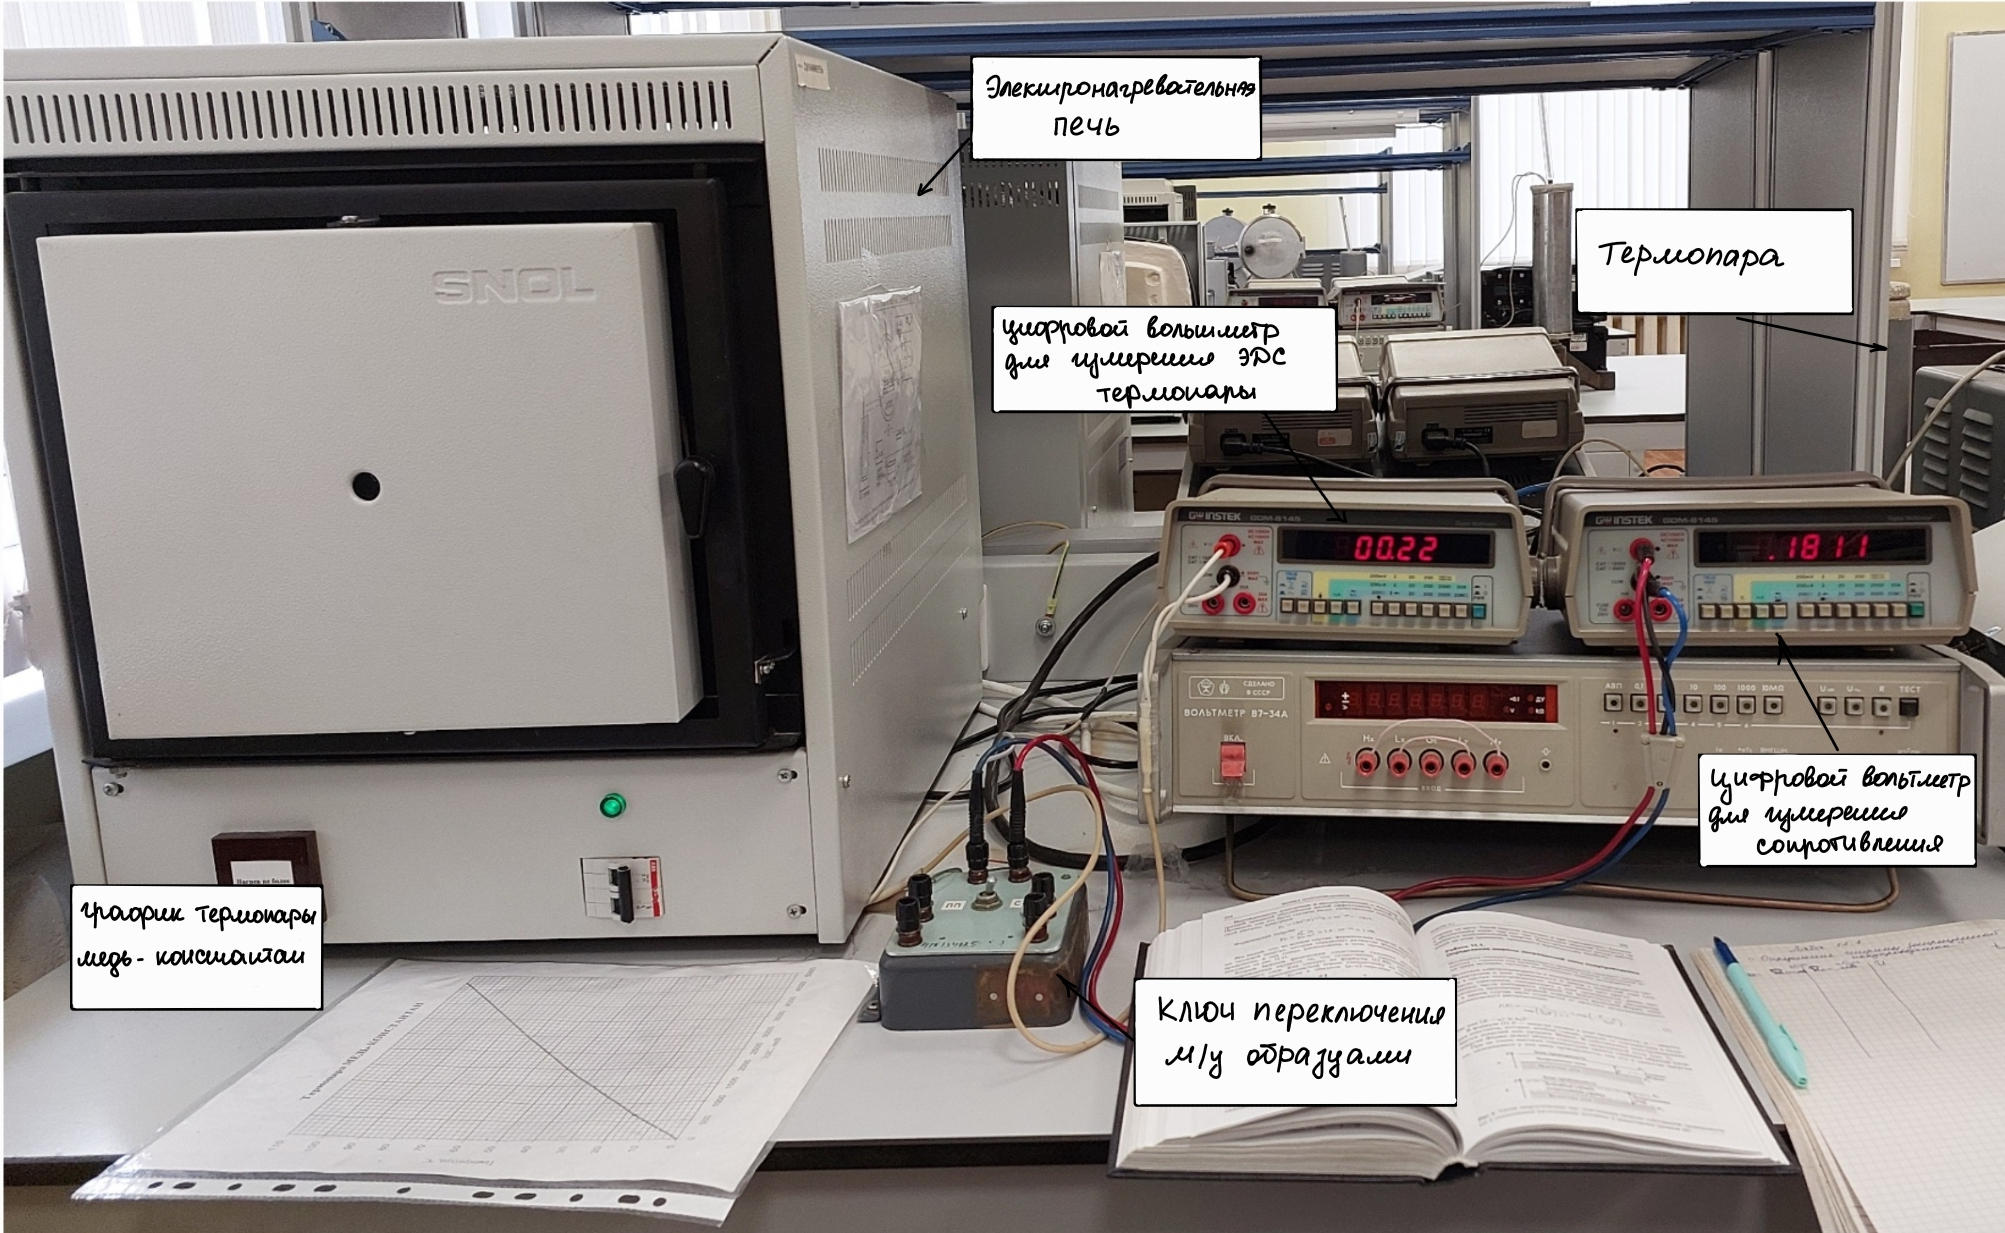
\includegraphics[width = 0.7 \linewidth]{ustanovka.jpg}
    \captionof{figure}{ Установка по измерению зависимости $\sigma(T)$}
    \label{ustanovka_real}
\end{center}

Параметры рассматриваемых образцов: 
\begin{itemize}
    \item Медный образец: $l = 13,4$ м; $d = 0,07$ мм 
    \item Полупроводникый образец: $a = c = 4,1$ мм; $b = 39,2$ мм
\end{itemize}

В режиме измерения сопротивления на пределах 1 кОм погрешность в процентах не превышает 
\begin{equation*}
    \pm[0,015\pm0,02(R_{k}/R_{x} - 1)],
\end{equation*}
где $R_{k}$ - включенный предел измерений, $R_{x}$ - значение измеряемой величины в килоомах.

Постоянная термопары равна $41 \cdot 10^{-6}$ В/К.

\section*{4. Результаты эксперимента и обработка данных}

Запишем параметры образцов:
\begin{itemize}
    \item $l_{Cu}$ = 13.4 мм
    \item $S_{Cu} = 4.9 \cdot 10^{-3} \text{ мм}^{2}$
    \item $l_{pp}$ = 39.2 мм
    \item $S_{pp} = 16.81 \text{ мм}^{2}$
\end{itemize}

Используем график термопары медь-константан для перевода показаний вольтметра в градусы (см. рис. \ref{graph}):

\begin{center}
    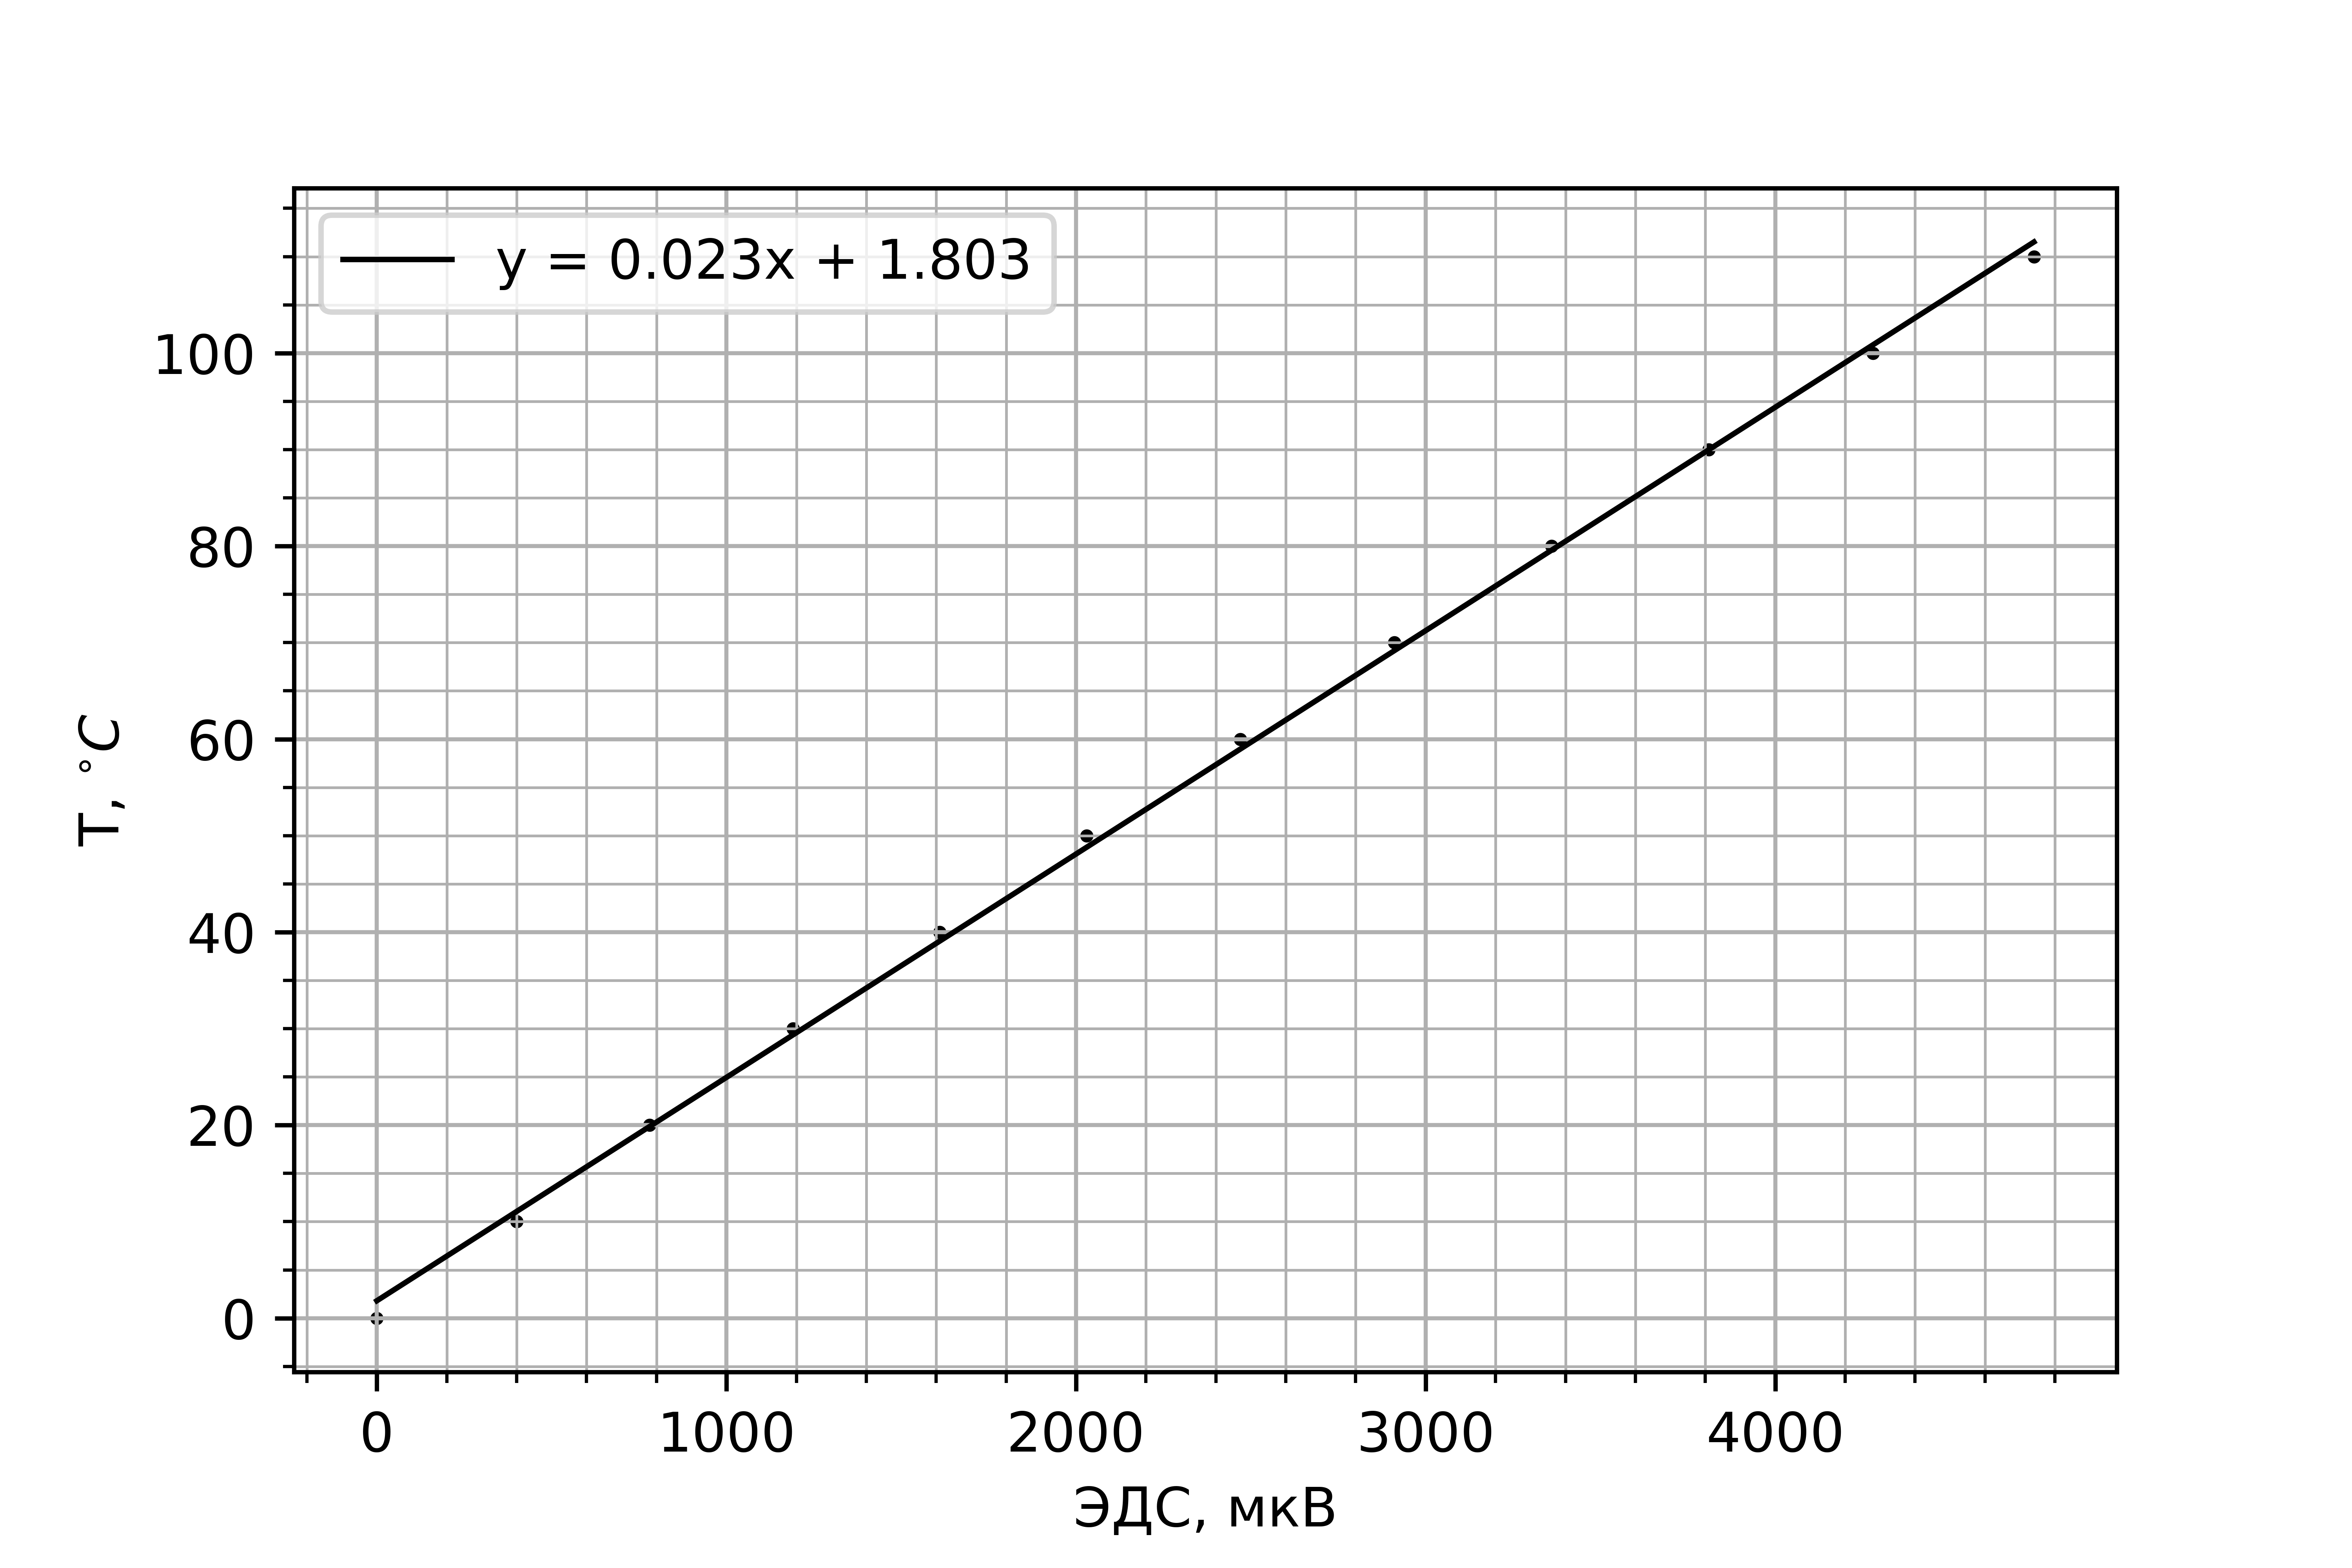
\includegraphics[width = 0.7 \linewidth]{graph.png}
    \captionof{figure}{Градуировочный график медь-константан}
    \label{graph}
\end{center}

Измерим зависимость удельной теплопроводности полупроводника и металла от температуры (см. таблицы \ref{table_cu} и \ref{table_pp} ) и построим соответствующие графики (рис. \ref{медь} и рис. \ref{полупроводник}):

\begin{center}
    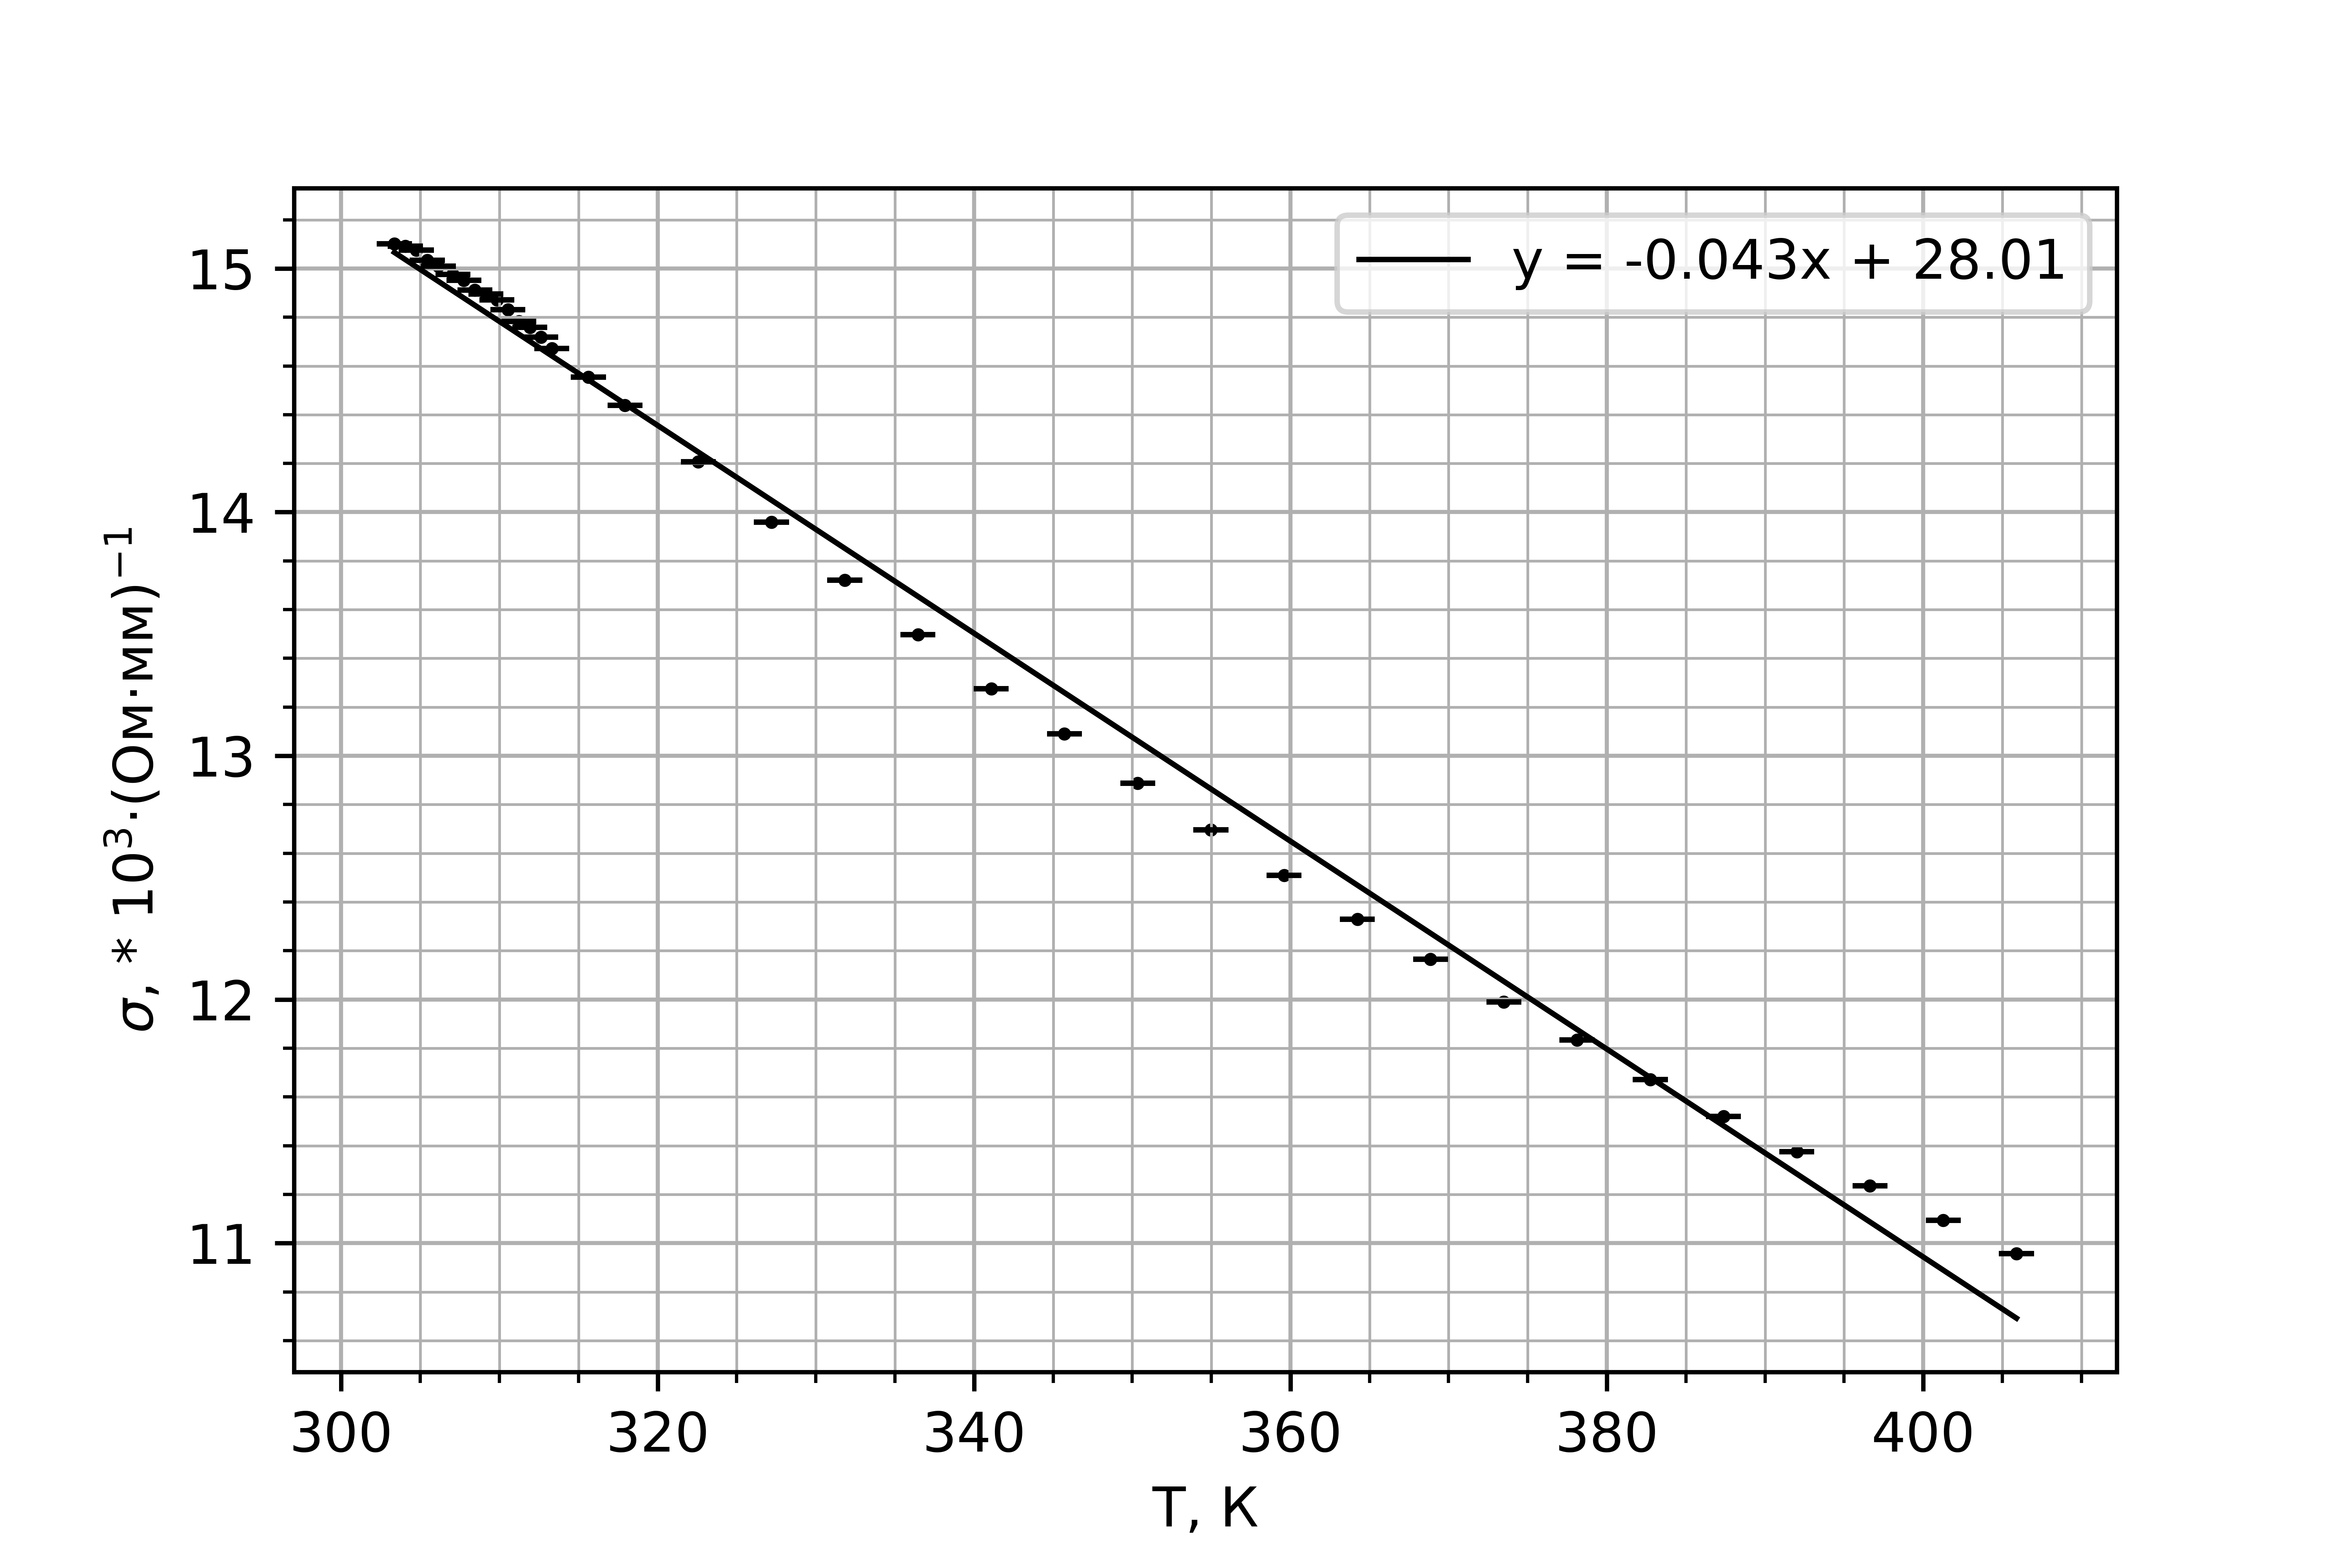
\includegraphics[width = 0.7 \linewidth]{sigma_Cu(T).png}
    \captionof{figure}{Зависимость $\sigma(T)$ для медного образца}
    \label{медь}
\end{center}

\begin{center}
    \includegraphics[width = 0.7 \linewidth]{sigma_пп(T).png}
    \captionof{figure}{Зависимость $\sigma(T)$ для полупроводникового образца}
    \label{полупроводник}
\end{center}

Таким образом, исходя из данных графика \ref{медь}, определим температурный коэффициент сопротивления меди по наклону графика.

Температурный коэффициент сопротивления определяется следующим образом: 
\begin{equation*}
    \alpha = \frac{1}{R}\frac{dR}{dT} = \frac{\sigma S}{l}\frac{d}{dT}\Big(\frac{l}{\sigma S} \Big) = -\frac{1}{\sigma}\frac{d\sigma}{dT}= (31,79\pm 0,91) \cdot 10^{3} \text{ К}^{-1}
\end{equation*}

Как видно из графиков, $\sigma$ для меди уменьшается линейно, в то время как у полупроводника её значение экспоненциально возрастает (аппроксимировали полиномом 4 степени $y = 2.36\cdot10^{-7} x^{4} - 2.51\cdot10^{-4} x^{3} + 0.11x^{2} - 20.95x + 1683$ ). Свойства проводимости металлов хорошо описываются \textit{моделью свободных электронов}: в отсутствие внешних полей электроны движутся с постоянной скоростью прямолинейно, столкновения считаются мгновенными. В большом диапазоне температур  получаем зависимость проводимости для металлов $\sigma \propto 1/T$ 

В то же время для полупроводника условием протекания тока является попадание электрона в зону проводимости, и вероятность электрона оказаться там экспоненциально зависит от температуры: $\sigma \propto \exp{\Big(-\frac{\Delta}{2kT}\Big)}$

Для полупроводникового образца построим график $ln(\sigma) = f(\frac{1}{T})$ (см.рис \ref{ширина запрещенной зоны} и таблицу \ref{sigma}). 

\begin{center}
    \includegraphics[width = 0.7 \linewidth]{ln(sigma_пп).png}
    \captionof{figure}{Зависимость $ln(\sigma)(1/T)$ для полупроводникового образца}
    \label{ширина запрещенной зоны}
\end{center}

По наклону его линейной части найдем ширину запрещенной зоны:
\begin{equation*}
    \Delta = -2kk_{\text{Б}} = (0.71 \pm 0.05) \text{ эВ}
\end{equation*}

Найденное значение в пределах $\sigma$ соответствует ширине запрещенной зоны \textbf{германия} (табл. $\Delta_{Ge} = 0,70$ эВ) при температурах порядка 300 К

\section*{5. Вывод}

В работе были исследованы проводимости металла и полупроводника в зависимости от температуры - результаты согласуются с теорией. В количественные оценки входили:
\begin{itemize}
    \item значение температурного коэффициента сопротивления меди: $\alpha = (31,79\pm 0,91) \cdot 10^{3} \text{ К}^{-1}$ 
    \item значение ширины запрещенной зоны полупроводника, материал которого нужно было определить: $\Delta = 0,71 \pm 0,05 \text{ эВ}$, что соответствует табличным данным для германия.
\end{itemize}


\newpage
\section*{6. Приложение}

\begin{table}[h!]
\begin{tabular}{|c|c|c|c|c|c|}
\hline
$R_{Cu}$, Ом  &  $U$,мВ & $T$, К  & $\sigma_{T}$, К           & $\sigma_{Cu}, \cdot 10^{3} \cdot (\text{Ом}\cdot\text{мм})^{-1}$ & $\sigma_{\sigma_{Cu}}, \cdot 10^{3} \cdot (\text{Ом}\cdot\text{мм})^{-1}$  \\ \hline
181,1     & 0,24 & 303,4 & \multirow{36}{*}{1,1} & 15,10                            & \multirow{36}{*}{0,01}                 \\ \cline{1-3} \cline{5-5}
181,2     & 0,27 & 304,1 &                       & 15,09                            &                                        \\ \cline{1-3} \cline{5-5}
181,4     & 0,30 & 304,7 &                       & 15,08                            &                                        \\ \cline{1-3} \cline{5-5}
181,9     & 0,33 & 305,4 &                       & 15,03                            &                                        \\ \cline{1-3} \cline{5-5}
182,2     & 0,36 & 306,1 &                       & 15,01                            &                                        \\ \cline{1-3} \cline{5-5}
182,6     & 0,40 & 307,1 &                       & 14,98                            &                                        \\ \cline{1-3} \cline{5-5}
182,9     & 0,43 & 307,8 &                       & 14,95                            &                                        \\ \cline{1-3} \cline{5-5}
183,4     & 0,46 & 308,5 &                       & 14,91                            &                                        \\ \cline{1-3} \cline{5-5}
183,6     & 0,49 & 309,1 &                       & 14,89                            &                                        \\ \cline{1-3} \cline{5-5}
183,9     & 0,52 & 309,8 &                       & 14,87                            &                                        \\ \cline{1-3} \cline{5-5}
184,4     & 0,55 & 310,5 &                       & 14,83                            &                                        \\ \cline{1-3} \cline{5-5}
185       & 0,58 & 311,2 &                       & 14,78                            &                                        \\ \cline{1-3} \cline{5-5}
185,3     & 0,61 & 311,9 &                       & 14,76                            &                                        \\ \cline{1-3} \cline{5-5}
185,8     & 0,64 & 312,6 &                       & 14,72                            &                                        \\ \cline{1-3} \cline{5-5}
186,4     & 0,67 & 313,3 &                       & 14,67                            &                                        \\ \cline{1-3} \cline{5-5}
187,9     & 0,77 & 315,6 &                       & 14,55                            &                                        \\ \cline{1-3} \cline{5-5}
189,4     & 0,87 & 317,9 &                       & 14,44                            &                                        \\ \cline{1-3} \cline{5-5}
192,5     & 1,07 & 322,6 &                       & 14,21                            &                                        \\ \cline{1-3} \cline{5-5}
195,9     & 1,27 & 327,2 &                       & 13,96                            &                                        \\ \cline{1-3} \cline{5-5}
199,3     & 1,47 & 331,8 &                       & 13,72                            &                                        \\ \cline{1-3} \cline{5-5}
202,6     & 1,67 & 336,5 &                       & 13,50                            &                                        \\ \cline{1-3} \cline{5-5}
206       & 1,87 & 341,1 &                       & 13,28                            &                                        \\ \cline{1-3} \cline{5-5}
208,9     & 2,07 & 345,7 &                       & 13,09                            &                                        \\ \cline{1-3} \cline{5-5}
212,2     & 2,27 & 350,3 &                       & 12,89                            &                                        \\ \cline{1-3} \cline{5-5}
215,4     & 2,47 & 355,0 &                       & 12,70                            &                                        \\ \cline{1-3} \cline{5-5}
218,6     & 2,67 & 359,6 &                       & 12,51                            &                                        \\ \cline{1-3} \cline{5-5}
221,8     & 2,87 & 364,2 &                       & 12,33                            &                                        \\ \cline{1-3} \cline{5-5}
224,8     & 3,07 & 368,9 &                       & 12,17                            &                                        \\ \cline{1-3} \cline{5-5}
228,1     & 3,27 & 373,5 &                       & 11,99                            &                                        \\ \cline{1-3} \cline{5-5}
231,1     & 3,47 & 378,1 &                       & 11,83                            &                                        \\ \cline{1-3} \cline{5-5}
234,3     & 3,67 & 382,7 &                       & 11,67                            &                                        \\ \cline{1-3} \cline{5-5}
237,4     & 3,87 & 387,4 &                       & 11,52                            &                                        \\ \cline{1-3} \cline{5-5}
240,4     & 4,07 & 392,0 &                       & 11,38                            &                                        \\ \cline{1-3} \cline{5-5}
243,4     & 4,27 & 396,6 &                       & 11,24                            &                                        \\ \cline{1-3} \cline{5-5}
246,5     & 4,47 & 401,3 &                       & 11,09                            &                                        \\ \cline{1-3} \cline{5-5}
249,6     & 4,67 & 405,9 &                       & 10,96                            &                                        \\ \hline
\end{tabular}
\caption{Результаты измерений зависимости $\sigma_{Cu}(T)$}
\label{table_cu}
\end{table}

\begin{table}[h!]
\begin{tabular}{|c|c|c|c|c|c|}
\hline
$R_{\text{пп}}$, Ом  &  $U$,мВ & $T$, К  & $\sigma_{T}$, К           & $\sigma_{\text{пп}}, \cdot 10^{3} \cdot (\text{Ом}\cdot\text{мм})^{-1}$ & $\sigma_{\sigma_{\text{пп}}}, \cdot 10^{3} \cdot (\text{Ом}\cdot\text{мм})^{-1}$\\ \hline
287,6     & 0,24 & 303,4 & \multirow{36}{*}{1,1} & 8,11      & \multirow{20}{*}{0,01} \\ \cline{1-3} \cline{5-5}
286,4     & 0,27 & 304,1 &                       & 8,14      &                        \\ \cline{1-3} \cline{5-5}
285,1     & 0,30 & 304,7 &                       & 8,18      &                        \\ \cline{1-3} \cline{5-5}
282,7     & 0,33 & 305,4 &                       & 8,25      &                        \\ \cline{1-3} \cline{5-5}
281,1     & 0,36 & 306,1 &                       & 8,30      &                        \\ \cline{1-3} \cline{5-5}
277,8     & 0,40 & 307,1 &                       & 8,39      &                        \\ \cline{1-3} \cline{5-5}
276,2     & 0,43 & 307,8 &                       & 8,44      &                        \\ \cline{1-3} \cline{5-5}
273,3     & 0,46 & 308,5 &                       & 8,53      &                        \\ \cline{1-3} \cline{5-5}
272       & 0,49 & 309,1 &                       & 8,57      &                        \\ \cline{1-3} \cline{5-5}
269,4     & 0,52 & 309,8 &                       & 8,66      &                        \\ \cline{1-3} \cline{5-5}
265,4     & 0,55 & 310,5 &                       & 8,79      &                        \\ \cline{1-3} \cline{5-5}
261,8     & 0,58 & 311,2 &                       & 8,91      &                        \\ \cline{1-3} \cline{5-5}
258,1     & 0,61 & 311,9 &                       & 9,04      &                        \\ \cline{1-3} \cline{5-5}
255,6     & 0,64 & 312,6 &                       & 9,12      &                        \\ \cline{1-3} \cline{5-5}
250,9     & 0,67 & 313,3 &                       & 9,29      &                        \\ \cline{1-3} \cline{5-5}
238       & 0,77 & 315,6 &                       & 9,80      &                        \\ \cline{1-3} \cline{5-5}
225,7     & 0,87 & 317,9 &                       & 10,33     &                        \\ \cline{1-3} \cline{5-5}
196,2     & 1,07 & 322,6 &                       & 11,89     &                        \\ \cline{1-3} \cline{5-5}
168       & 1,27 & 327,2 &                       & 13,88     &                        \\ \cline{1-3} \cline{5-5}
143,4     & 1,47 & 331,8 &                       & 16,26     &                        \\ \cline{1-3} \cline{5-6} 
121,5     & 1,67 & 336,5 &                       & 19,19     & \multirow{2}{*}{0,02}  \\ \cline{1-3} \cline{5-5}
102,1     & 1,87 & 341,1 &                       & 22,84     &                        \\ \cline{1-3} \cline{5-6} 
87,1      & 2,07 & 345,7 &                       & 26,77     & 0,03                   \\ \cline{1-3} \cline{5-6} 
74,2      & 2,27 & 350,3 &                       & 31,43     & 0,04                   \\ \cline{1-3} \cline{5-6} 
63,5      & 2,47 & 355,0 &                       & 36,72     & 0,06                   \\ \cline{1-3} \cline{5-6} 
54,3      & 2,67 & 359,6 &                       & 42,95     & 0,08                   \\ \cline{1-3} \cline{5-6} 
46,8      & 2,87 & 364,2 &                       & 49,83     & 0,11                   \\ \cline{1-3} \cline{5-6} 
40,7      & 3,07 & 368,9 &                       & 57,30     & 0,14                   \\ \cline{1-3} \cline{5-6} 
35,2      & 3,27 & 373,5 &                       & 66,25     & 0,19                   \\ \cline{1-3} \cline{5-6} 
30,9      & 3,47 & 378,1 &                       & 75,47     & 0,24                   \\ \cline{1-3} \cline{5-6} 
27,1      & 3,67 & 382,7 &                       & 86,05     & 0,32                   \\ \cline{1-3} \cline{5-6} 
23,8      & 3,87 & 387,4 &                       & 97,98     & 0,41                   \\ \cline{1-3} \cline{5-6} 
21,1      & 4,07 & 392,0 &                       & 110,52    & 0,52                   \\ \cline{1-3} \cline{5-6} 
18,7      & 4,27 & 396,6 &                       & 124,70    & 0,67                   \\ \cline{1-3} \cline{5-6} 
16,7      & 4,47 & 401,3 &                       & 139,64    & 0,84                   \\ \cline{1-3} \cline{5-6} 
14,9      & 4,67 & 405,9 &                       & 156,51    & 1,05                   \\ \hline
\end{tabular}
\caption{Результаты измерений зависимости $\sigma_{\text{пп}}(T)$}
\label{table_pp}
\end{table}

\begin{table}[h!]
\begin{tabular}{|c|c|c|c|}
\hline
$\ln\sigma$ & $\sigma_{\ln\sigma}$        & $\frac{1}{T}, \text{К}^{-1}$  & $\sigma_{\frac{1}{T}}, \text{К}^{-1}$              \\ \hline
2,09      & \multirow{36}{*}{0,01} & 3,30 & \multirow{36}{*}{0,01} \\ \cline{1-1} \cline{3-3}
2,10      &                        & 3,29 &                        \\ \cline{1-1} \cline{3-3}
2,10      &                        & 3,28 &                        \\ \cline{1-1} \cline{3-3}
2,11      &                        & 3,27 &                        \\ \cline{1-1} \cline{3-3}
2,12      &                        & 3,27 &                        \\ \cline{1-1} \cline{3-3}
2,13      &                        & 3,26 &                        \\ \cline{1-1} \cline{3-3}
2,13      &                        & 3,25 &                        \\ \cline{1-1} \cline{3-3}
2,14      &                        & 3,24 &                        \\ \cline{1-1} \cline{3-3}
2,15      &                        & 3,23 &                        \\ \cline{1-1} \cline{3-3}
2,16      &                        & 3,23 &                        \\ \cline{1-1} \cline{3-3}
2,17      &                        & 3,22 &                        \\ \cline{1-1} \cline{3-3}
2,19      &                        & 3,21 &                        \\ \cline{1-1} \cline{3-3}
2,20      &                        & 3,21 &                        \\ \cline{1-1} \cline{3-3}
2,21      &                        & 3,20 &                        \\ \cline{1-1} \cline{3-3}
2,23      &                        & 3,19 &                        \\ \cline{1-1} \cline{3-3}
2,28      &                        & 3,17 &                        \\ \cline{1-1} \cline{3-3}
2,34      &                        & 3,15 &                        \\ \cline{1-1} \cline{3-3}
2,48      &                        & 3,10 &                        \\ \cline{1-1} \cline{3-3}
2,63      &                        & 3,06 &                        \\ \cline{1-1} \cline{3-3}
2,79      &                        & 3,01 &                        \\ \cline{1-1} \cline{3-3}
2,95      &                        & 2,97 &                        \\ \cline{1-1} \cline{3-3}
3,13      &                        & 2,93 &                        \\ \cline{1-1} \cline{3-3}
3,29      &                        & 2,89 &                        \\ \cline{1-1} \cline{3-3}
3,45      &                        & 2,85 &                        \\ \cline{1-1} \cline{3-3}
3,60      &                        & 2,82 &                        \\ \cline{1-1} \cline{3-3}
3,76      &                        & 2,78 &                        \\ \cline{1-1} \cline{3-3}
3,91      &                        & 2,75 &                        \\ \cline{1-1} \cline{3-3}
4,05      &                        & 2,71 &                        \\ \cline{1-1} \cline{3-3}
4,19      &                        & 2,68 &                        \\ \cline{1-1} \cline{3-3}
4,32      &                        & 2,64 &                        \\ \cline{1-1} \cline{3-3}
4,45      &                        & 2,61 &                        \\ \cline{1-1} \cline{3-3}
4,58      &                        & 2,58 &                        \\ \cline{1-1} \cline{3-3}
4,71      &                        & 2,55 &                        \\ \cline{1-1} \cline{3-3}
4,83      &                        & 2,52 &                        \\ \cline{1-1} \cline{3-3}
4,94      &                        & 2,49 &                        \\ \cline{1-1} \cline{3-3}
5,05      &                        & 2,46 &                        \\ \hline
\end{tabular}
\caption{Данные графика зависимости $ln\sigma(\frac{1}{T})$}
\label{sigma}
\end{table}

\end{document}
